%
% Copyright (c) 2011-2013, fortiss GmbH.
% Licensed under the Apache License, Version 2.0.
% 
% Use, modification and distribution are subject to the terms specified
% in the accompanying license file LICENSE.txt located at the root directory
% of this software distribution. A copy is available at
% http://chromosome.fortiss.org/.
%
% This file is part of CHROMOSOME.
%
% $Id$
%

\section{Installing the Modeling Tool}
\label{appx:install_xmt}

\subsection{Installation}

The \xme Modeling Tool (XMT) is provided as an Eclipse plugin.
fortiss provides an Eclipse update-site at \url{http://download.fortiss.org/public/xme/xmt/update-site/} from where you can install it.
This section will first describe how to install Eclipse and then describe how to install the XMT plugin from the update-site.\footnote{%
	When you visit he update-site with your browser a web page will appear with a link to the Eclipse help site for installing from update-sites.
}
%
Let us start with the installation of Eclipse:

\begin{enumerate}
	\item The XMT requires Eclipse Indigo. 
More recent versions are not supported and may not be fully compatible.
To download the correct version of Eclipse,
point your favorite browser to the following web page:\\
\url{http://www.eclipse.org/downloads/packages/eclipse-modeling-tools/indigosr2}\\
and click on the link corresponding to your operating system to download Eclipse.
The linked version is the Eclipse Modeling Tools package and already contains several of the plugins required by the XMT.
	\item After downloading you simply extract the Eclipse archive into a directory of your choice.
	\item If you do not already have a Java Runtime Environment installed, then go to the following web page and do this now
		(install the product named \emph{Java SE Development Kit} found in the \emph{Java Platform (JDK)} category):\\
\url{http://www.oracle.com/technetwork/java/javase/downloads/}\\
		\textbf{Notice that you need at least Java version 1.7!}\\
		Also make sure that the versions of Java and Eclipse match (32-bit/64-bit).
	\item Go into the Eclipse directory and start the Eclipse executable.
		When asked for a workspace directory, either accept the proposed location or enter a directory of your choice.
		Eclipse will store your settings and projects in that directory.
\end{enumerate}
%
Now we can install the XMT plugin into Eclipse.

\begin{enumerate}
	\item In Eclipse select \textit{Help $\rightarrow$ Install New Software...}. This will show the install dialog. 
	\item Click on the \texttt{Add...} button and enter as location:\\
\url{http://download.fortiss.org/public/xme/xmt/update-site/}\\
and press \texttt{OK}. Loading may take some time.
	\item You will see a long list of categories. Select the category '\xme Modeling Tool (XMT)'.\footnote{%
		All other plugins that are needed by the tool are included in this update-site and will be installed automatically.
	}
	\item Make sure that you have the same options selected as in Figure~\ref{fig:xmt_update-site.png}.
	\item Press \texttt{Next} to continue. Eclipse will show that it is about to install the XMT plugin. There shouldn't be any errors.
	\item Press \texttt{Next} again. The licenses of the XMT plugin will be displayed.
If you want to continue you must accept it and press \texttt{Finish}. This will start the installation.
	\item During installation Eclipse will warn about unsigned content. Press \texttt{OK} to continue.
	\item After the installation you will be prompted to restart Eclipse. Do this and you are done.
\end{enumerate}

\begin{figure}[htpb]
	\centering
	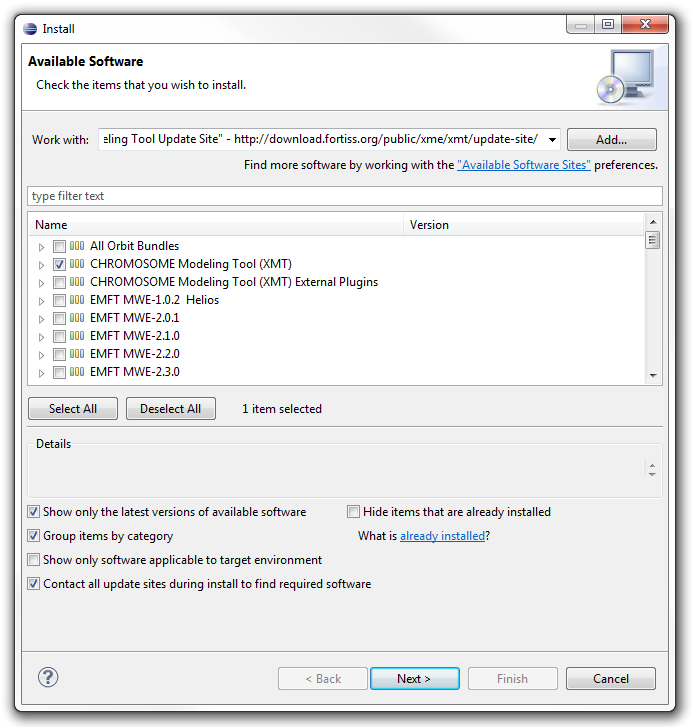
\includegraphics[scale=0.5]{figures/xmt_update-site.png}
	\caption{Install dialog of XMT update-site.}
	\label{fig:xmt_update-site.png}
\end{figure}

To verify if the tool has been installed correctly go to \textit{Window $\rightarrow$ Open Perspective $\rightarrow$ Other...}. You should see an entry 'XMT'.

\subsection{Troubleshooting}

\begin{itemize}
	\item The XMT perspective is not visible after installation of the XMT plugin.
	\begin{itemize}
		\item Check if you have at least Java Runtime 1.7 installed.
		If you have several java versions installed, then also check if eclipse is run with the correct one.
		To force eclipse to use a certain version you can add the following two lines to the \texttt{eclipse.ini}\footnote{You find this file directly in your eclipse installation directory.} file:
		\begin{verbatim}
			-vm
			C:/path/to/java/bin/javaw.exe
		\end{verbatim}
		Replace the second line with your actual path to the java executable.
		Note that you \emph{must} enter it in two separate lines like above.
		You must also put it before the \texttt{-vmargs} option.
	\end{itemize}
\end{itemize}